%%%%%%%%%%%%%%%%%%%%%%%%
% Boost
%%%%%%%%%%%%%%%%%%%%%%%%

\subsubsection{Purpose}
\noindent \ac{EMTG} depends on three components of Boost: filesystem, serialization, and system (and their dependencies). In addition, if a user wishes to build the \ac{EMTG} PyHardware and Propulator components, then the python component of Boost is required. \\ \ac{EMTG} is known to work with \hl{Boost 1.79.0}.

\subsubsection{Bundled Installation Instructions}
\begin{enumerate}
	\item Open the \textless EMTG-root\textgreater \textbackslash depend\textbackslash boost directory.
	\item Confirm that the sub-directories contain files.
	\item If the files exist, proceed to Step~\ref{bundle:boost} of Section~\ref{sec:boost_installation_instructions}. \\ If for some reason the files do not exist, go to the next sub-section to download it.
\end{enumerate}

\subsubsection{Download Location}
\noindent The main page for the software distributions is in the following website: \\
\url{https://www.boost.org/users/download/}

\noindent The software package needed for the EMTG version indicated in this guide can be obtained from the following location: \\
\emph{(In the event the url is no longer active, navigate to the aforementioned software website to find the specific version)} \\
\url{https://sourceforge.net/projects/boost/files/boost-binaries/1.79.0/boost_1_79_0-msvc-14.3-64.exe/download/}

\noindent \hl{Executing the Boost installer requires elevated privileges.}

\subsubsection{Dependency Installation Instructions}
\label{sec:boost_installation_instructions}
\begin{enumerate}
	\item Execute the downloaded file and proceed through the install instructions utilizing the defaults unless otherwise indicated in the following steps 
	\begin{enumerate}
		\item When prompted for the install location, save to a destination with no spaces in the file path (e.g. C:\textbackslash SW\_Installs\textbackslash boost\_1\_79\_0) and record its location for future use
	\end{enumerate}
	\item \label{bundle:boost} Creation of a “user-config.jam” file in your home directory
	\begin{enumerate}
		\item Navigate to your user directory (e.g. “C:\textbackslash Users\textbackslash MyName\textbackslash”)
		\item Create a “user-config.jam” file
		\item Copy the following contents to the file: \\
		\begin{verbatim}
			using python : 3.7 ; 
			using python : : C:\\Path\\To\\python.exe ;
		\end{verbatim}	
		\item 
			Replace ``\texttt{C:\textbackslash Path\textbackslash To\textbackslash python.exe}'' with the PyEmtgEnv environment that 
			contains the python 3.7 executable then save the file \\
			(e.g. \texttt{C:\textbackslash Users\textbackslash MyName\textbackslash mambaforge\textbackslash envs\textbackslash PyEmtgEnv\textbackslash python.exe})
		\\ \\
		Note that the white space is important! \\ For additional information, see the Boost documentation at \url{https://www.boost.org/doc/libs/1_79_0/libs/python/doc/html/building/configuring_boost_build.html}.
	\end{enumerate}	
	\item Open a Visual Studio Developer Command Prompt 
		\begin{figure}[H]
			\centering
			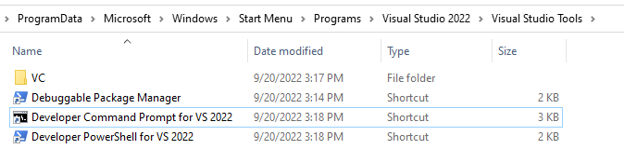
\includegraphics[width=0.9\linewidth]{../../../shared_latex_inputs/images/vstudio_cprompt_launch.png}
			\caption{Visual Studio Command Prompt Launch Icon}
		\end{figure}
	\begin{enumerate}
		\item Click the Start menu button
		\item Click on the `Visual Studio *' folder 
		\item Select the `Developer Command Prompt *' option
	\end{enumerate}
	\item Navigate to the root Boost directory (e.g. \textless EMTG-root\textgreater \textbackslash depend \textbackslash boost or C:\textbackslash SW\_Installs\textbackslash boost\_1\_79\_0) in the command window
	\item Type the following and hit Enter:
	\begin{verbatim}
		bootstrap
	\end{verbatim}	
	\item Type the following, all on one line, and hit Enter:
	\begin{verbatim}
		.\b2 address-model=64 link=static threading=multi runtime-link=shared 
		
		--with-filesystem --with-serialization --with-system --with-python
	\end{verbatim} \\ \\
	If successful, the Boost root directory should now contain the directory path stage\textbackslash lib\textbackslash, and there should be several .lib files there. 
	\begin{figure}[H]
		\centering
		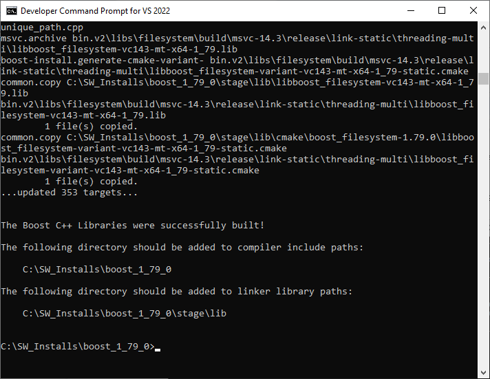
\includegraphics[width=0.7\linewidth]{../../../shared_latex_inputs/images/boost_build_success.png}
		\caption{Boost Successful Build Output}
	\end{figure}
\end{enumerate}
